\message{ !name(db_structure.tex)}
\message{ !name(db_structure.tex) !offset(-2) }
\section[Разработка структуры БД]{РАЗРАБОТКА СТРУКТУРЫ БАЗЫ ДАННЫХ}
\label{sub:db_structure}

Задача проектирования базы данных (БД) в целом формулируется
следующим образом: выбрать подходящую логическую структуру для заданного
массива данных, которые требуется поместить в базу данных~\cite{date05}.

Перечислим основные цели проектирования баз данных:
\begin{itemize}
\item
  обеспечение хранения в БД всех необходимых данных;
\item
  обеспечение получения данных по всем необходимым запросам;
\item
  сокращение избыточности и дублирования данных;
\item
  обеспечение целостности данных: исключение потери данных, противоречий в
  содержании БД, нарушений смысла данных;
\item
  сокращение времени обработки запросов к данным.
\end{itemize}

В этом разделе рассматривается процесс проектирования базы данных разрабатываемого
веб-сервиса.
В подразделе~\ref{ssub:db_structure_stages} описываются основные этапы проектирования
баз данных в целом.
Подразделы~\ref{ssub:db_info_stage},~\ref{ssub:db_data_stage},~\ref{ssub:db_physical_stage}
подробно описывают каждый из этапов проектирования базы данных разрабатываемого веб-сервиса.

\subsection{Этапы проектирования базы данных}
\label{ssub:db_structure_stages}

В процессе проектирования баз данных выделяют три основных этапа:
\begin{itemize}
\item инфологическое проектирование;
\item даталогическое проектирование;
\item физическое проектирование;
\end{itemize}

Рассмотрим каждый из этих этапов более подробно.

\textit{Инфологическое (концептуальное) проектирование} --- анализ
предметной области и ее описание. Этот этап осуществляется без ориентации
на какие-либо конкретные программные или технические средства реализации.
Результатом инфологического проектирования является \textit{инфологическая модель} ---
формализованная модель предметной области, построенная с использованием
специальных языковых средств (обычно графических).

Инфологическая модель включает следующие основные элементы:
\begin{itemize}
\item
  описание объектов предметной области;
\item
  описание атрибутов (свойств) объектов;
\item
  описание связей между объектами.
\end{itemize}

Для описания объектов предметной области, их атрибутов и связей между
ними обычно применяются стандартизированные системы графических обозначений.
Кроме того, инфологическая модель может включать
описание основных запросов к проектируемой БД,
описание документов, используемых в качестве
источников данных для БД или составляемых на основе БД,
описание алгоритмических связей между данными,
описание ограничений целостности, т.е. правил, обеспечивающих
актуальность и непротиворечивость данных.

Для описания объектов предметной области и связей между ними
могут использоваться модели <<сущность-связь>> (\textit{ER-модели}).

\textit{Даталогическое (логическое) проектирование} --- описание
логической структуры данных средствами системы управления базами данных
(СУБД), для которой проектируется БД.
Такое описание (\textit{даталогическая модель}) строится на основе инфологической модели
по определенным правилам.
Для реляционных БД даталогическая модель состоит из следующих частей:
\begin{itemize}
\item
  описания таблиц;
\item
  описания связей между таблицами;
\item
  описания атрибутов.
\end{itemize}

\textit{Физическое проектирование} --- на этом этапе выполняется описание физической
структуры БД, то есть ее размещения на запоминающем устройстве.
Такое описание называется \textit{физической моделью}, которая включает:

\begin{itemize}
\item
  тип носителя;
\item
  способы организации данных;
\item
  способы управления свободной памятью;
\item
  способы сжатия данных и т.д.
\end{itemize}

\subsection{Инфологическое проектирование}
\label{ssub:db_info_stage}

Разрабатываемый сервис должен хранить и предоставлять в наглядной форме 
информацию о государственных наградах РБ и лицах, которые были ими награждены.
Более формально, сервис должен по запросу пользователей выполнять следующие операции:
\begin{itemize}
\item
  предоставление доступа к хранимой информации: генерация html-страниц с данными
  о запрашиваемых наградах или награжденных лицах;
\item
  расчет и наглядное представление статистических показателей на основе хранимых данных;
\item
  предоставление информации о награжденных в машиночитаемом формате для последующего 
  загрузки на носитель пользователя. 
\end{itemize}

Кроме этого, администратор сервиса должен иметь возможность загрузки данных в базу данных
из файла машиночитаемого формата, а также возможность редактирования содержимого БД
через графический интерфейс, предоставляемый сервисом.

На рисунке~\ref{fig:use-case_diagram} представлена диаграмма сценариев
использования проектируемого сервиса.

\begin{figure}[h!]
  \centering
  \small{
    % Graphic for TeX using PGF
% Title: /home/budnyjj/univer/GIT/discipline/BIBD/course_b/project/uml/use-case.dia
% Creator: Dia v0.97.2
% CreationDate: Mon May 19 14:11:38 2014
% For: budnyjj
% \usepackage{tikz}
% The following commands are not supported in PSTricks at present
% We define them conditionally, so when they are implemented,
% this pgf file will use them.
\ifx\du\undefined
  \newlength{\du}
\fi
\setlength{\du}{15\unitlength}
\begin{tikzpicture}
\pgftransformxscale{1.000000}
\pgftransformyscale{-1.000000}
\definecolor{dialinecolor}{rgb}{0.000000, 0.000000, 0.000000}
\pgfsetstrokecolor{dialinecolor}
\definecolor{dialinecolor}{rgb}{1.000000, 1.000000, 1.000000}
\pgfsetfillcolor{dialinecolor}
\pgfsetlinewidth{0.100000\du}
\pgfsetdash{}{0pt}
\definecolor{dialinecolor}{rgb}{1.000000, 1.000000, 1.000000}
\pgfsetfillcolor{dialinecolor}
\pgfpathellipse{\pgfpoint{8.300000\du}{4.950000\du}}{\pgfpoint{0.300000\du}{0\du}}{\pgfpoint{0\du}{0.300000\du}}
\pgfusepath{fill}
\definecolor{dialinecolor}{rgb}{0.000000, 0.000000, 0.000000}
\pgfsetstrokecolor{dialinecolor}
\pgfpathellipse{\pgfpoint{8.300000\du}{4.950000\du}}{\pgfpoint{0.300000\du}{0\du}}{\pgfpoint{0\du}{0.300000\du}}
\pgfusepath{stroke}
\definecolor{dialinecolor}{rgb}{0.000000, 0.000000, 0.000000}
\pgfsetstrokecolor{dialinecolor}
\draw (7.100000\du,5.550000\du)--(9.500000\du,5.550000\du);
\definecolor{dialinecolor}{rgb}{0.000000, 0.000000, 0.000000}
\pgfsetstrokecolor{dialinecolor}
\draw (8.300000\du,5.250000\du)--(8.300000\du,6.750000\du);
\definecolor{dialinecolor}{rgb}{0.000000, 0.000000, 0.000000}
\pgfsetstrokecolor{dialinecolor}
\draw (8.300000\du,6.750000\du)--(7.100000\du,8.050000\du);
\definecolor{dialinecolor}{rgb}{0.000000, 0.000000, 0.000000}
\pgfsetstrokecolor{dialinecolor}
\draw (8.300000\du,6.750000\du)--(9.500000\du,8.050000\du);
% setfont left to latex
\definecolor{dialinecolor}{rgb}{0.000000, 0.000000, 0.000000}
\pgfsetstrokecolor{dialinecolor}
\node at (8.300000\du,9.245000\du){Пользователь};
\pgfsetlinewidth{0.100000\du}
\pgfsetdash{}{0pt}
\definecolor{dialinecolor}{rgb}{1.000000, 1.000000, 1.000000}
\pgfsetfillcolor{dialinecolor}
\pgfpathellipse{\pgfpoint{8.100000\du}{13.550001\du}}{\pgfpoint{0.300000\du}{0\du}}{\pgfpoint{0\du}{0.300000\du}}
\pgfusepath{fill}
\definecolor{dialinecolor}{rgb}{0.000000, 0.000000, 0.000000}
\pgfsetstrokecolor{dialinecolor}
\pgfpathellipse{\pgfpoint{8.100000\du}{13.550001\du}}{\pgfpoint{0.300000\du}{0\du}}{\pgfpoint{0\du}{0.300000\du}}
\pgfusepath{stroke}
\definecolor{dialinecolor}{rgb}{0.000000, 0.000000, 0.000000}
\pgfsetstrokecolor{dialinecolor}
\draw (6.900000\du,14.150001\du)--(9.300000\du,14.150001\du);
\definecolor{dialinecolor}{rgb}{0.000000, 0.000000, 0.000000}
\pgfsetstrokecolor{dialinecolor}
\draw (8.100000\du,13.850001\du)--(8.100000\du,15.350001\du);
\definecolor{dialinecolor}{rgb}{0.000000, 0.000000, 0.000000}
\pgfsetstrokecolor{dialinecolor}
\draw (8.100000\du,15.350001\du)--(6.900000\du,16.650001\du);
\definecolor{dialinecolor}{rgb}{0.000000, 0.000000, 0.000000}
\pgfsetstrokecolor{dialinecolor}
\draw (8.100000\du,15.350001\du)--(9.300000\du,16.650001\du);
% setfont left to latex
\definecolor{dialinecolor}{rgb}{0.000000, 0.000000, 0.000000}
\pgfsetstrokecolor{dialinecolor}
\node at (8.100000\du,17.845001\du){Администратор};
\pgfsetlinewidth{0.100000\du}
\pgfsetdash{}{0pt}
\pgfsetmiterjoin
\pgfsetbuttcap
{
\definecolor{dialinecolor}{rgb}{0.000000, 0.000000, 0.000000}
\pgfsetfillcolor{dialinecolor}
% was here!!!
\definecolor{dialinecolor}{rgb}{0.000000, 0.000000, 0.000000}
\pgfsetstrokecolor{dialinecolor}
\draw (10.660214\du,6.750000\du)--(13.050000\du,6.750000\du)--(13.050000\du,8.892500\du)--(15.150000\du,8.892500\du);
}
% setfont left to latex
\definecolor{dialinecolor}{rgb}{0.000000, 0.000000, 0.000000}
\pgfsetstrokecolor{dialinecolor}
\node[anchor=west] at (13.150000\du,7.671250\du){};
\definecolor{dialinecolor}{rgb}{0.000000, 0.000000, 0.000000}
\pgfsetfillcolor{dialinecolor}
\fill (13.250000\du,7.671250\du)--(13.250000\du,7.271250\du)--(13.650000\du,7.471250\du)--cycle;
\definecolor{dialinecolor}{rgb}{0.000000, 0.000000, 0.000000}
\pgfsetstrokecolor{dialinecolor}
\node[anchor=west] at (10.860214\du,6.600000\du){};
\definecolor{dialinecolor}{rgb}{0.000000, 0.000000, 0.000000}
\pgfsetstrokecolor{dialinecolor}
\node[anchor=east] at (14.950000\du,8.742500\du){};
\pgfsetlinewidth{0.100000\du}
\pgfsetdash{}{0pt}
\pgfsetmiterjoin
\pgfsetbuttcap
{
\definecolor{dialinecolor}{rgb}{0.000000, 0.000000, 0.000000}
\pgfsetfillcolor{dialinecolor}
% was here!!!
\definecolor{dialinecolor}{rgb}{0.000000, 0.000000, 0.000000}
\pgfsetstrokecolor{dialinecolor}
\draw (10.660214\du,6.750000\du)--(13.050000\du,6.750000\du)--(13.050000\du,4.700000\du)--(16.899999\du,4.700000\du);
}
% setfont left to latex
\definecolor{dialinecolor}{rgb}{0.000000, 0.000000, 0.000000}
\pgfsetstrokecolor{dialinecolor}
\node[anchor=west] at (13.150000\du,5.575000\du){};
\definecolor{dialinecolor}{rgb}{0.000000, 0.000000, 0.000000}
\pgfsetfillcolor{dialinecolor}
\fill (13.250000\du,5.575000\du)--(13.250000\du,5.175000\du)--(13.650000\du,5.375000\du)--cycle;
\definecolor{dialinecolor}{rgb}{0.000000, 0.000000, 0.000000}
\pgfsetstrokecolor{dialinecolor}
\node[anchor=west] at (10.860214\du,6.600000\du){};
\definecolor{dialinecolor}{rgb}{0.000000, 0.000000, 0.000000}
\pgfsetstrokecolor{dialinecolor}
\node[anchor=east] at (16.699999\du,4.550000\du){};
\pgfsetlinewidth{0.100000\du}
\pgfsetdash{}{0pt}
\pgfsetmiterjoin
\pgfsetbuttcap
{
\definecolor{dialinecolor}{rgb}{0.000000, 0.000000, 0.000000}
\pgfsetfillcolor{dialinecolor}
% was here!!!
\definecolor{dialinecolor}{rgb}{0.000000, 0.000000, 0.000000}
\pgfsetstrokecolor{dialinecolor}
\draw (10.753967\du,15.350001\du)--(13.000000\du,15.350001\du)--(13.000000\du,13.165001\du)--(16.300444\du,13.165001\du);
}
% setfont left to latex
\definecolor{dialinecolor}{rgb}{0.000000, 0.000000, 0.000000}
\pgfsetstrokecolor{dialinecolor}
\node[anchor=west] at (13.100000\du,14.107501\du){};
\definecolor{dialinecolor}{rgb}{0.000000, 0.000000, 0.000000}
\pgfsetfillcolor{dialinecolor}
\fill (13.200000\du,14.107501\du)--(13.200000\du,13.707501\du)--(13.600000\du,13.907501\du)--cycle;
\definecolor{dialinecolor}{rgb}{0.000000, 0.000000, 0.000000}
\pgfsetstrokecolor{dialinecolor}
\node[anchor=west] at (10.953967\du,15.200001\du){};
\definecolor{dialinecolor}{rgb}{0.000000, 0.000000, 0.000000}
\pgfsetstrokecolor{dialinecolor}
\node[anchor=east] at (16.100444\du,13.015001\du){};
\pgfsetlinewidth{0.100000\du}
\pgfsetdash{}{0pt}
\pgfsetmiterjoin
\pgfsetbuttcap
{
\definecolor{dialinecolor}{rgb}{0.000000, 0.000000, 0.000000}
\pgfsetfillcolor{dialinecolor}
% was here!!!
\definecolor{dialinecolor}{rgb}{0.000000, 0.000000, 0.000000}
\pgfsetstrokecolor{dialinecolor}
\draw (10.753967\du,15.350001\du)--(13.000000\du,15.350001\du)--(13.000000\du,17.618334\du)--(15.099831\du,17.618334\du);
}
% setfont left to latex
\definecolor{dialinecolor}{rgb}{0.000000, 0.000000, 0.000000}
\pgfsetstrokecolor{dialinecolor}
\node[anchor=west] at (13.100000\du,16.334167\du){};
\definecolor{dialinecolor}{rgb}{0.000000, 0.000000, 0.000000}
\pgfsetfillcolor{dialinecolor}
\fill (13.200000\du,16.334167\du)--(13.200000\du,15.934167\du)--(13.600000\du,16.134167\du)--cycle;
\definecolor{dialinecolor}{rgb}{0.000000, 0.000000, 0.000000}
\pgfsetstrokecolor{dialinecolor}
\node[anchor=west] at (10.953967\du,15.200001\du){};
\definecolor{dialinecolor}{rgb}{0.000000, 0.000000, 0.000000}
\pgfsetstrokecolor{dialinecolor}
\node[anchor=east] at (14.899831\du,17.468334\du){};
\pgfsetlinewidth{0.100000\du}
\pgfsetdash{}{0pt}
\pgfsetdash{}{0pt}
\pgfsetmiterjoin
\definecolor{dialinecolor}{rgb}{0.000000, 0.000000, 0.000000}
\pgfsetstrokecolor{dialinecolor}
\draw (11.800000\du,2.750000\du)--(11.800000\du,20.302696\du)--(29.500000\du,20.302696\du)--(29.500000\du,2.750000\du)--cycle;
% setfont left to latex
\definecolor{dialinecolor}{rgb}{0.000000, 0.000000, 0.000000}
\pgfsetstrokecolor{dialinecolor}
\node at (20.650000\du,11.721348\du){};
\pgfsetlinewidth{0.100000\du}
\pgfsetdash{}{0pt}
\definecolor{dialinecolor}{rgb}{1.000000, 1.000000, 1.000000}
\pgfsetfillcolor{dialinecolor}
\pgfpathellipse{\pgfpoint{21.579999\du}{4.700000\du}}{\pgfpoint{4.680000\du}{0\du}}{\pgfpoint{0\du}{1.600000\du}}
\pgfusepath{fill}
\definecolor{dialinecolor}{rgb}{0.000000, 0.000000, 0.000000}
\pgfsetstrokecolor{dialinecolor}
\pgfpathellipse{\pgfpoint{21.579999\du}{4.700000\du}}{\pgfpoint{4.680000\du}{0\du}}{\pgfpoint{0\du}{1.600000\du}}
\pgfusepath{stroke}
% setfont left to latex
\definecolor{dialinecolor}{rgb}{0.000000, 0.000000, 0.000000}
\pgfsetstrokecolor{dialinecolor}
\node at (21.579999\du,4.495000\du){Просмотр};
% setfont left to latex
\definecolor{dialinecolor}{rgb}{0.000000, 0.000000, 0.000000}
\pgfsetstrokecolor{dialinecolor}
\node at (21.579999\du,5.295000\du){ html-страниц};
\pgfsetlinewidth{0.100000\du}
\pgfsetdash{}{0pt}
\definecolor{dialinecolor}{rgb}{1.000000, 1.000000, 1.000000}
\pgfsetfillcolor{dialinecolor}
\pgfpathellipse{\pgfpoint{21.577500\du}{8.892500\du}}{\pgfpoint{6.427500\du}{0\du}}{\pgfpoint{0\du}{2.142500\du}}
\pgfusepath{fill}
\definecolor{dialinecolor}{rgb}{0.000000, 0.000000, 0.000000}
\pgfsetstrokecolor{dialinecolor}
\pgfpathellipse{\pgfpoint{21.577500\du}{8.892500\du}}{\pgfpoint{6.427500\du}{0\du}}{\pgfpoint{0\du}{2.142500\du}}
\pgfusepath{stroke}
% setfont left to latex
\definecolor{dialinecolor}{rgb}{0.000000, 0.000000, 0.000000}
\pgfsetstrokecolor{dialinecolor}
\node at (21.577500\du,8.687500\du){Загрузка данных};
% setfont left to latex
\definecolor{dialinecolor}{rgb}{0.000000, 0.000000, 0.000000}
\pgfsetstrokecolor{dialinecolor}
\node at (21.577500\du,9.487500\du){на локальный носитель};
\pgfsetlinewidth{0.100000\du}
\pgfsetdash{}{0pt}
\definecolor{dialinecolor}{rgb}{1.000000, 1.000000, 1.000000}
\pgfsetfillcolor{dialinecolor}
\pgfpathellipse{\pgfpoint{21.645000\du}{13.165001\du}}{\pgfpoint{5.295000\du}{0\du}}{\pgfpoint{0\du}{1.765000\du}}
\pgfusepath{fill}
\definecolor{dialinecolor}{rgb}{0.000000, 0.000000, 0.000000}
\pgfsetstrokecolor{dialinecolor}
\pgfpathellipse{\pgfpoint{21.645000\du}{13.165001\du}}{\pgfpoint{5.295000\du}{0\du}}{\pgfpoint{0\du}{1.765000\du}}
\pgfusepath{stroke}
% setfont left to latex
\definecolor{dialinecolor}{rgb}{0.000000, 0.000000, 0.000000}
\pgfsetstrokecolor{dialinecolor}
\node at (21.645000\du,12.960001\du){Редактирование };
% setfont left to latex
\definecolor{dialinecolor}{rgb}{0.000000, 0.000000, 0.000000}
\pgfsetstrokecolor{dialinecolor}
\node at (21.645000\du,13.760001\du){содержимого БД};
\pgfsetlinewidth{0.100000\du}
\pgfsetdash{}{0pt}
\definecolor{dialinecolor}{rgb}{1.000000, 1.000000, 1.000000}
\pgfsetfillcolor{dialinecolor}
\pgfpathellipse{\pgfpoint{21.655000\du}{17.618334\du}}{\pgfpoint{6.505000\du}{0\du}}{\pgfpoint{0\du}{2.168333\du}}
\pgfusepath{fill}
\definecolor{dialinecolor}{rgb}{0.000000, 0.000000, 0.000000}
\pgfsetstrokecolor{dialinecolor}
\pgfpathellipse{\pgfpoint{21.655000\du}{17.618334\du}}{\pgfpoint{6.505000\du}{0\du}}{\pgfpoint{0\du}{2.168333\du}}
\pgfusepath{stroke}
% setfont left to latex
\definecolor{dialinecolor}{rgb}{0.000000, 0.000000, 0.000000}
\pgfsetstrokecolor{dialinecolor}
\node at (21.655000\du,17.413334\du){Импорт данных в БД };
% setfont left to latex
\definecolor{dialinecolor}{rgb}{0.000000, 0.000000, 0.000000}
\pgfsetstrokecolor{dialinecolor}
\node at (21.655000\du,18.213334\du){из локального носителя};
% setfont left to latex
\definecolor{dialinecolor}{rgb}{0.000000, 0.000000, 0.000000}
\pgfsetstrokecolor{dialinecolor}
\node[anchor=west] at (21.577500\du,8.892500\du){};
\end{tikzpicture}

  }
  \caption{Диаграмма сценариев использования проектируемого веб-сервиса}
  \label{fig:use-case_diagram}
\end{figure}

В качестве источника данных используются файлы в машиночитаемом формате,
которые получаются после разбора соответствующих файлов формата pdf,
предоставленных национальным статистическим
комитетом Республики Беларусь.

Файлы-источники данных имеют формат csv или xml c заранее определенным
набором cтолбцов, который не может подвергаться изменениям.
В качестве формата файлов, предоставляемых пользователям для загрузки,
также используются csv либо xml.

На рисунке~\ref{fig:activity_diagram} представлены потоки обработки данных,
имеющих отношение к проектируемому веб-сервису.

\begin{figure}[h!]
  \centering
  \small{
    % Graphic for TeX using PGF
% Title: /home/budnyjj/univer/GIT/discipline/BIBD/course_b/project/uml/activity.dia
% Creator: Dia v0.97.2
% CreationDate: Thu May  1 13:14:33 2014
% For: budnyjj
% \usepackage{tikz}
% The following commands are not supported in PSTricks at present
% We define them conditionally, so when they are implemented,
% this pgf file will use them.
\ifx\du\undefined
  \newlength{\du}
\fi
\setlength{\du}{15\unitlength}
\begin{tikzpicture}
\pgftransformxscale{1.000000}
\pgftransformyscale{-1.000000}
\definecolor{dialinecolor}{rgb}{0.000000, 0.000000, 0.000000}
\pgfsetstrokecolor{dialinecolor}
\definecolor{dialinecolor}{rgb}{1.000000, 1.000000, 1.000000}
\pgfsetfillcolor{dialinecolor}
\pgfsetlinewidth{0.100000\du}
\pgfsetdash{}{0pt}
\definecolor{dialinecolor}{rgb}{0.000000, 0.000000, 0.000000}
\pgfsetfillcolor{dialinecolor}
\pgfpathellipse{\pgfpoint{13.250000\du}{2.150000\du}}{\pgfpoint{0.500000\du}{0\du}}{\pgfpoint{0\du}{0.500000\du}}
\pgfusepath{fill}
\pgfsetlinewidth{0.100000\du}
\pgfsetdash{}{0pt}
{\pgfsetcornersarced{\pgfpoint{1.000000\du}{1.000000\du}}\definecolor{dialinecolor}{rgb}{1.000000, 1.000000, 1.000000}
\pgfsetfillcolor{dialinecolor}
\fill (8.500000\du,5.200000\du)--(8.500000\du,7.800000\du)--(18.045000\du,7.800000\du)--(18.045000\du,5.200000\du)--cycle;
}{\pgfsetcornersarced{\pgfpoint{1.000000\du}{1.000000\du}}\definecolor{dialinecolor}{rgb}{0.000000, 0.000000, 0.000000}
\pgfsetstrokecolor{dialinecolor}
\draw (8.500000\du,5.200000\du)--(8.500000\du,7.800000\du)--(18.045000\du,7.800000\du)--(18.045000\du,5.200000\du)--cycle;
}% setfont left to latex
\definecolor{dialinecolor}{rgb}{0.000000, 0.000000, 0.000000}
\pgfsetstrokecolor{dialinecolor}
\node at (13.272500\du,6.295000\du){Разбор содержимого pdf,};
% setfont left to latex
\definecolor{dialinecolor}{rgb}{0.000000, 0.000000, 0.000000}
\pgfsetstrokecolor{dialinecolor}
\node at (13.272500\du,7.095000\du){генерация csv, xml};
\pgfsetlinewidth{0.100000\du}
\pgfsetbuttcap
\pgfsetdash{}{0pt}
{
\definecolor{dialinecolor}{rgb}{0.000000, 0.000000, 0.000000}
\pgfsetfillcolor{dialinecolor}
% was here!!!
\pgfsetarrowsend{to}
\definecolor{dialinecolor}{rgb}{0.000000, 0.000000, 0.000000}
\pgfsetstrokecolor{dialinecolor}
\draw (13.250000\du,2.700269\du)--(13.250000\du,3.950134\du)--(13.272500\du,3.950134\du)--(13.272500\du,5.200000\du);
}
% setfont left to latex
\pgfsetlinewidth{0.100000\du}
\pgfsetdash{}{0pt}
\definecolor{dialinecolor}{rgb}{1.000000, 1.000000, 1.000000}
\pgfsetfillcolor{dialinecolor}
\fill (15.350000\du,0.550000\du)--(26.815000\du,0.550000\du)--(27.415000\du,1.150000\du)--(27.415000\du,3.850000\du)--(15.350000\du,3.850000\du)--cycle;
\definecolor{dialinecolor}{rgb}{0.000000, 0.000000, 0.000000}
\pgfsetstrokecolor{dialinecolor}
\draw (15.350000\du,0.550000\du)--(26.815000\du,0.550000\du)--(27.415000\du,1.150000\du)--(27.415000\du,3.850000\du)--(15.350000\du,3.850000\du)--cycle;
\pgfsetlinewidth{0.050000\du}
\definecolor{dialinecolor}{rgb}{0.000000, 0.000000, 0.000000}
\pgfsetstrokecolor{dialinecolor}
\draw (26.815000\du,0.550000\du)--(26.815000\du,1.150000\du)--(27.415000\du,1.150000\du);
% setfont left to latex
\definecolor{dialinecolor}{rgb}{0.000000, 0.000000, 0.000000}
\pgfsetstrokecolor{dialinecolor}
\node[anchor=west] at (15.700000\du,1.795000\du){Данные национального};
% setfont left to latex
\definecolor{dialinecolor}{rgb}{0.000000, 0.000000, 0.000000}
\pgfsetstrokecolor{dialinecolor}
\node[anchor=west] at (15.700000\du,2.595000\du){статистического комитета РБ,};
% setfont left to latex
\definecolor{dialinecolor}{rgb}{0.000000, 0.000000, 0.000000}
\pgfsetstrokecolor{dialinecolor}
\node[anchor=west] at (15.700000\du,3.395000\du){предоставленные в формате pdf};
\pgfsetlinewidth{0.100000\du}
\pgfsetdash{{1.000000\du}{1.000000\du}}{0\du}
\pgfsetdash{{0.400000\du}{0.400000\du}}{0\du}
\pgfsetmiterjoin
\pgfsetbuttcap
{
\definecolor{dialinecolor}{rgb}{0.498039, 0.498039, 0.498039}
\pgfsetfillcolor{dialinecolor}
% was here!!!
\pgfsetarrowsend{to}
\definecolor{dialinecolor}{rgb}{0.498039, 0.498039, 0.498039}
\pgfsetstrokecolor{dialinecolor}
\draw (15.350000\du,2.200000\du)--(14.775134\du,2.200000\du)--(14.775134\du,2.150000\du)--(13.800269\du,2.150000\du);
}
% setfont left to latex
\pgfsetlinewidth{0.100000\du}
\pgfsetbuttcap
\pgfsetdash{}{0pt}
{
\definecolor{dialinecolor}{rgb}{0.000000, 0.000000, 0.000000}
\pgfsetfillcolor{dialinecolor}
% was here!!!
\pgfsetarrowsend{to}
\definecolor{dialinecolor}{rgb}{0.000000, 0.000000, 0.000000}
\pgfsetstrokecolor{dialinecolor}
\draw (13.272500\du,7.800000\du)--(13.272500\du,10.150000\du)--(8.407500\du,10.150000\du)--(8.407500\du,12.050000\du);
}
% setfont left to latex
\pgfsetlinewidth{0.100000\du}
\pgfsetbuttcap
\pgfsetdash{}{0pt}
{
\definecolor{dialinecolor}{rgb}{0.000000, 0.000000, 0.000000}
\pgfsetfillcolor{dialinecolor}
% was here!!!
\pgfsetarrowsend{to}
\definecolor{dialinecolor}{rgb}{0.000000, 0.000000, 0.000000}
\pgfsetstrokecolor{dialinecolor}
\draw (13.272500\du,7.800000\du)--(13.272500\du,10.150000\du)--(17.587500\du,10.150000\du)--(17.587500\du,12.150000\du);
}
% setfont left to latex
\pgfsetlinewidth{0.100000\du}
\pgfsetdash{}{0pt}
{\pgfsetcornersarced{\pgfpoint{1.000000\du}{1.000000\du}}\definecolor{dialinecolor}{rgb}{1.000000, 1.000000, 1.000000}
\pgfsetfillcolor{dialinecolor}
\fill (5.150000\du,12.050000\du)--(5.150000\du,14.650000\du)--(11.665000\du,14.650000\du)--(11.665000\du,12.050000\du)--cycle;
}{\pgfsetcornersarced{\pgfpoint{1.000000\du}{1.000000\du}}\definecolor{dialinecolor}{rgb}{0.000000, 0.000000, 0.000000}
\pgfsetstrokecolor{dialinecolor}
\draw (5.150000\du,12.050000\du)--(5.150000\du,14.650000\du)--(11.665000\du,14.650000\du)--(11.665000\du,12.050000\du)--cycle;
}% setfont left to latex
\definecolor{dialinecolor}{rgb}{0.000000, 0.000000, 0.000000}
\pgfsetstrokecolor{dialinecolor}
\node at (8.407500\du,13.145000\du){Импорт данных };
% setfont left to latex
\definecolor{dialinecolor}{rgb}{0.000000, 0.000000, 0.000000}
\pgfsetstrokecolor{dialinecolor}
\node at (8.407500\du,13.945000\du){о наградах};
\pgfsetlinewidth{0.100000\du}
\pgfsetdash{}{0pt}
{\pgfsetcornersarced{\pgfpoint{1.000000\du}{1.000000\du}}\definecolor{dialinecolor}{rgb}{1.000000, 1.000000, 1.000000}
\pgfsetfillcolor{dialinecolor}
\fill (14.250000\du,12.150000\du)--(14.250000\du,14.750000\du)--(20.925000\du,14.750000\du)--(20.925000\du,12.150000\du)--cycle;
}{\pgfsetcornersarced{\pgfpoint{1.000000\du}{1.000000\du}}\definecolor{dialinecolor}{rgb}{0.000000, 0.000000, 0.000000}
\pgfsetstrokecolor{dialinecolor}
\draw (14.250000\du,12.150000\du)--(14.250000\du,14.750000\du)--(20.925000\du,14.750000\du)--(20.925000\du,12.150000\du)--cycle;
}% setfont left to latex
\definecolor{dialinecolor}{rgb}{0.000000, 0.000000, 0.000000}
\pgfsetstrokecolor{dialinecolor}
\node at (17.587500\du,13.245000\du){Импорт данных };
% setfont left to latex
\definecolor{dialinecolor}{rgb}{0.000000, 0.000000, 0.000000}
\pgfsetstrokecolor{dialinecolor}
\node at (17.587500\du,14.045000\du){о награжденных};
\pgfsetlinewidth{0.100000\du}
\pgfsetdash{}{0pt}
\definecolor{dialinecolor}{rgb}{1.000000, 1.000000, 1.000000}
\pgfsetfillcolor{dialinecolor}
\fill (19.350000\du,7.800000\du)--(27.350000\du,7.800000\du)--(27.950000\du,8.400000\du)--(27.950000\du,9.500000\du)--(19.350000\du,9.500000\du)--cycle;
\definecolor{dialinecolor}{rgb}{0.000000, 0.000000, 0.000000}
\pgfsetstrokecolor{dialinecolor}
\draw (19.350000\du,7.800000\du)--(27.350000\du,7.800000\du)--(27.950000\du,8.400000\du)--(27.950000\du,9.500000\du)--(19.350000\du,9.500000\du)--cycle;
\pgfsetlinewidth{0.050000\du}
\definecolor{dialinecolor}{rgb}{0.000000, 0.000000, 0.000000}
\pgfsetstrokecolor{dialinecolor}
\draw (27.350000\du,7.800000\du)--(27.350000\du,8.400000\du)--(27.950000\du,8.400000\du);
% setfont left to latex
\definecolor{dialinecolor}{rgb}{0.000000, 0.000000, 0.000000}
\pgfsetstrokecolor{dialinecolor}
\node[anchor=west] at (19.700000\du,9.045000\du){awarded (.csv, .xml)};
\pgfsetlinewidth{0.100000\du}
\pgfsetdash{}{0pt}
\definecolor{dialinecolor}{rgb}{1.000000, 1.000000, 1.000000}
\pgfsetfillcolor{dialinecolor}
\fill (0.800000\du,7.550000\du)--(8.415000\du,7.550000\du)--(9.015000\du,8.150000\du)--(9.015000\du,9.250000\du)--(0.800000\du,9.250000\du)--cycle;
\definecolor{dialinecolor}{rgb}{0.000000, 0.000000, 0.000000}
\pgfsetstrokecolor{dialinecolor}
\draw (0.800000\du,7.550000\du)--(8.415000\du,7.550000\du)--(9.015000\du,8.150000\du)--(9.015000\du,9.250000\du)--(0.800000\du,9.250000\du)--cycle;
\pgfsetlinewidth{0.050000\du}
\definecolor{dialinecolor}{rgb}{0.000000, 0.000000, 0.000000}
\pgfsetstrokecolor{dialinecolor}
\draw (8.415000\du,7.550000\du)--(8.415000\du,8.150000\du)--(9.015000\du,8.150000\du);
% setfont left to latex
\definecolor{dialinecolor}{rgb}{0.000000, 0.000000, 0.000000}
\pgfsetstrokecolor{dialinecolor}
\node[anchor=west] at (1.150000\du,8.795000\du){awards (.csv, .xml)};
\pgfsetlinewidth{0.100000\du}
\pgfsetdash{{0.400000\du}{0.400000\du}}{0\du}
\pgfsetdash{{0.400000\du}{0.400000\du}}{0\du}
\pgfsetmiterjoin
\pgfsetbuttcap
{
\definecolor{dialinecolor}{rgb}{0.498039, 0.498039, 0.498039}
\pgfsetfillcolor{dialinecolor}
% was here!!!
\pgfsetarrowsend{to}
\definecolor{dialinecolor}{rgb}{0.498039, 0.498039, 0.498039}
\pgfsetstrokecolor{dialinecolor}
\draw (9.015000\du,8.400000\du)--(10.350000\du,8.400000\du)--(10.350000\du,10.300000\du);
}
% setfont left to latex
\pgfsetlinewidth{0.100000\du}
\pgfsetdash{{0.400000\du}{0.400000\du}}{0\du}
\pgfsetdash{{0.400000\du}{0.400000\du}}{0\du}
\pgfsetmiterjoin
\pgfsetbuttcap
{
\definecolor{dialinecolor}{rgb}{0.498039, 0.498039, 0.498039}
\pgfsetfillcolor{dialinecolor}
% was here!!!
\pgfsetarrowsend{to}
\definecolor{dialinecolor}{rgb}{0.498039, 0.498039, 0.498039}
\pgfsetstrokecolor{dialinecolor}
\draw (19.350000\du,8.650000\du)--(17.250000\du,8.650000\du)--(17.250000\du,10.150000\du);
}
% setfont left to latex
\pgfsetlinewidth{0.100000\du}
\pgfsetdash{}{0pt}
\definecolor{dialinecolor}{rgb}{1.000000, 1.000000, 1.000000}
\pgfsetfillcolor{dialinecolor}
\fill (12.050000\du,17.000000\du)--(13.050000\du,16.000000\du)--(14.050000\du,17.000000\du)--(13.050000\du,18.000000\du)--cycle;
\definecolor{dialinecolor}{rgb}{0.498039, 0.498039, 0.498039}
\pgfsetstrokecolor{dialinecolor}
\draw (12.050000\du,17.000000\du)--(13.050000\du,16.000000\du)--(14.050000\du,17.000000\du)--(13.050000\du,18.000000\du)--cycle;
\pgfsetlinewidth{0.100000\du}
\pgfsetbuttcap
\pgfsetdash{}{0pt}
{
\definecolor{dialinecolor}{rgb}{0.000000, 0.000000, 0.000000}
\pgfsetfillcolor{dialinecolor}
% was here!!!
\pgfsetarrowsend{to}
\definecolor{dialinecolor}{rgb}{0.000000, 0.000000, 0.000000}
\pgfsetstrokecolor{dialinecolor}
\draw (8.407500\du,14.650000\du)--(8.400000\du,14.650000\du)--(8.400000\du,17.000000\du)--(12.050000\du,17.000000\du);
}
% setfont left to latex
\pgfsetlinewidth{0.100000\du}
\pgfsetbuttcap
\pgfsetdash{}{0pt}
{
\definecolor{dialinecolor}{rgb}{0.000000, 0.000000, 0.000000}
\pgfsetfillcolor{dialinecolor}
% was here!!!
\pgfsetarrowsend{to}
\definecolor{dialinecolor}{rgb}{0.000000, 0.000000, 0.000000}
\pgfsetstrokecolor{dialinecolor}
\draw (17.587500\du,14.750000\du)--(17.750000\du,14.750000\du)--(17.750000\du,17.000000\du)--(14.050000\du,17.000000\du);
}
% setfont left to latex
% setfont left to latex
\definecolor{dialinecolor}{rgb}{0.000000, 0.000000, 0.000000}
\pgfsetstrokecolor{dialinecolor}
\node[anchor=west] at (4.907500\du,8.400000\du){};
\pgfsetlinewidth{0.100000\du}
\pgfsetdash{}{0pt}
\definecolor{dialinecolor}{rgb}{1.000000, 1.000000, 1.000000}
\pgfsetfillcolor{dialinecolor}
\pgfpathellipse{\pgfpoint{13.400000\du}{26.000000\du}}{\pgfpoint{0.750000\du}{0\du}}{\pgfpoint{0\du}{0.750000\du}}
\pgfusepath{fill}
\definecolor{dialinecolor}{rgb}{0.000000, 0.000000, 0.000000}
\pgfsetstrokecolor{dialinecolor}
\pgfpathellipse{\pgfpoint{13.400000\du}{26.000000\du}}{\pgfpoint{0.750000\du}{0\du}}{\pgfpoint{0\du}{0.750000\du}}
\pgfusepath{stroke}
\definecolor{dialinecolor}{rgb}{0.000000, 0.000000, 0.000000}
\pgfsetfillcolor{dialinecolor}
\pgfpathellipse{\pgfpoint{13.400000\du}{26.000000\du}}{\pgfpoint{0.500000\du}{0\du}}{\pgfpoint{0\du}{0.500000\du}}
\pgfusepath{fill}
\pgfsetlinewidth{0.100000\du}
\pgfsetdash{}{0pt}
{\pgfsetcornersarced{\pgfpoint{1.000000\du}{1.000000\du}}\definecolor{dialinecolor}{rgb}{1.000000, 1.000000, 1.000000}
\pgfsetfillcolor{dialinecolor}
\fill (3.100000\du,20.150000\du)--(3.100000\du,24.350000\du)--(10.927500\du,24.350000\du)--(10.927500\du,20.150000\du)--cycle;
}{\pgfsetcornersarced{\pgfpoint{1.000000\du}{1.000000\du}}\definecolor{dialinecolor}{rgb}{0.000000, 0.000000, 0.000000}
\pgfsetstrokecolor{dialinecolor}
\draw (3.100000\du,20.150000\du)--(3.100000\du,24.350000\du)--(10.927500\du,24.350000\du)--(10.927500\du,20.150000\du)--cycle;
}% setfont left to latex
\definecolor{dialinecolor}{rgb}{0.000000, 0.000000, 0.000000}
\pgfsetstrokecolor{dialinecolor}
\node at (7.013750\du,21.245000\du){Генерация html};
% setfont left to latex
\definecolor{dialinecolor}{rgb}{0.000000, 0.000000, 0.000000}
\pgfsetstrokecolor{dialinecolor}
\node at (7.013750\du,22.045000\du){страниц с данными };
% setfont left to latex
\definecolor{dialinecolor}{rgb}{0.000000, 0.000000, 0.000000}
\pgfsetstrokecolor{dialinecolor}
\node at (7.013750\du,22.845000\du){о наградах };
% setfont left to latex
\definecolor{dialinecolor}{rgb}{0.000000, 0.000000, 0.000000}
\pgfsetstrokecolor{dialinecolor}
\node at (7.013750\du,23.645000\du){и награжденных};
\pgfsetlinewidth{0.100000\du}
\pgfsetbuttcap
\pgfsetdash{}{0pt}
{
\definecolor{dialinecolor}{rgb}{0.000000, 0.000000, 0.000000}
\pgfsetfillcolor{dialinecolor}
% was here!!!
\pgfsetarrowsend{to}
\definecolor{dialinecolor}{rgb}{0.000000, 0.000000, 0.000000}
\pgfsetstrokecolor{dialinecolor}
\draw (13.050000\du,18.000000\du)--(13.050000\du,19.075000\du)--(7.013750\du,19.075000\du)--(7.013750\du,20.150000\du);
}
% setfont left to latex
\pgfsetlinewidth{0.100000\du}
\pgfsetbuttcap
\pgfsetdash{}{0pt}
{
\definecolor{dialinecolor}{rgb}{0.000000, 0.000000, 0.000000}
\pgfsetfillcolor{dialinecolor}
% was here!!!
\pgfsetarrowsend{to}
\definecolor{dialinecolor}{rgb}{0.000000, 0.000000, 0.000000}
\pgfsetstrokecolor{dialinecolor}
\draw (7.013750\du,24.350000\du)--(7.013750\du,26.000000\du)--(12.599609\du,26.000000\du);
}
% setfont left to latex
\pgfsetlinewidth{0.100000\du}
\pgfsetdash{}{0pt}
{\pgfsetcornersarced{\pgfpoint{1.000000\du}{1.000000\du}}\definecolor{dialinecolor}{rgb}{1.000000, 1.000000, 1.000000}
\pgfsetfillcolor{dialinecolor}
\fill (15.200000\du,20.450000\du)--(15.200000\du,23.850000\du)--(26.515000\du,23.850000\du)--(26.515000\du,20.450000\du)--cycle;
}{\pgfsetcornersarced{\pgfpoint{1.000000\du}{1.000000\du}}\definecolor{dialinecolor}{rgb}{0.000000, 0.000000, 0.000000}
\pgfsetstrokecolor{dialinecolor}
\draw (15.200000\du,20.450000\du)--(15.200000\du,23.850000\du)--(26.515000\du,23.850000\du)--(26.515000\du,20.450000\du)--cycle;
}% setfont left to latex
\definecolor{dialinecolor}{rgb}{0.000000, 0.000000, 0.000000}
\pgfsetstrokecolor{dialinecolor}
\node at (20.857500\du,21.545000\du){Предоставление данных };
% setfont left to latex
\definecolor{dialinecolor}{rgb}{0.000000, 0.000000, 0.000000}
\pgfsetstrokecolor{dialinecolor}
\node at (20.857500\du,22.345000\du){о награжденных для загрузки};
% setfont left to latex
\definecolor{dialinecolor}{rgb}{0.000000, 0.000000, 0.000000}
\pgfsetstrokecolor{dialinecolor}
\node at (20.857500\du,23.145000\du){ в форматах xml либо csv};
\pgfsetlinewidth{0.100000\du}
\pgfsetbuttcap
\pgfsetdash{}{0pt}
{
\definecolor{dialinecolor}{rgb}{0.000000, 0.000000, 0.000000}
\pgfsetfillcolor{dialinecolor}
% was here!!!
\pgfsetarrowsend{to}
\definecolor{dialinecolor}{rgb}{0.000000, 0.000000, 0.000000}
\pgfsetstrokecolor{dialinecolor}
\draw (13.050000\du,17.950000\du)--(13.050000\du,19.100000\du)--(20.857500\du,19.100000\du)--(20.857500\du,20.450000\du);
}
% setfont left to latex
\pgfsetlinewidth{0.100000\du}
\pgfsetbuttcap
\pgfsetdash{}{0pt}
{
\definecolor{dialinecolor}{rgb}{0.000000, 0.000000, 0.000000}
\pgfsetfillcolor{dialinecolor}
% was here!!!
\pgfsetarrowsend{to}
\definecolor{dialinecolor}{rgb}{0.000000, 0.000000, 0.000000}
\pgfsetstrokecolor{dialinecolor}
\draw (20.857500\du,23.850000\du)--(20.857500\du,26.000000\du)--(14.150000\du,26.000000\du);
}
% setfont left to latex
% setfont left to latex
\definecolor{dialinecolor}{rgb}{0.000000, 0.000000, 0.000000}
\pgfsetstrokecolor{dialinecolor}
\node[anchor=west] at (19.750000\du,22.250000\du){};
% setfont left to latex
\definecolor{dialinecolor}{rgb}{0.000000, 0.000000, 0.000000}
\pgfsetstrokecolor{dialinecolor}
\node[anchor=west] at (4.907500\du,8.400000\du){};
\end{tikzpicture}

  }
  \caption{Диаграмма потоков данных проектируемого веб-сервиса}
  \label{fig:activity_diagram}
\end{figure}

Рассмотрим наборы данных, предоставляемых входными файлами.

Файл \textbf{awards.csv} хранит информацию о наградах и состоит из следующих полей:
\begin{itemize}
\item
  \textbf{award\_title} --- название награды
  (например, медаль <<За адзнаку ў воінскай службе>>);
\item
  \textbf{type} --- тип награды
  (медаль);
\item
  \textbf{description} --- краткое описание награды
  (медалем <<За адзнаку ў воінскай службе>>
  ўзнагароджваюцца вайскоўцы за значныя заслугі ў воінскай службе);
\end{itemize}

Атрибут \textbf{award\_title} является уникальным, поэтому его можно использовать
в качестве идентификатора награды.
Каждому типу \textbf{type} награды может соответствовать несколько названий 
(\textbf{award\_title}) и описаний (\textbf{description}).
Каждому названию (\textbf{award\_title}) или описанию (\textbf{description}) награды
соответствуетединственный тип \textbf{type}.
Содержимое полей атрибута \textbf{description} может отстутствовать.

Файл \textbf{awarded.csv} хранит информацию о награжденных и состоит из следующих полей:
\begin{itemize}
\item
  \textbf{fio} --- фамилия, имя, отчество награжденного
  (например, Апрышка Міхаіл Пятровіч);
\item
  \textbf{dolzhnost} --- занимаемая должность
  (галоўны інспектар аддзела арганізацыі мытнага кантролю Гомельская мытні);
\item
  \textbf{pol} --- пол награжденного
  (м);
\item
  \textbf{zvanie} --- звание;
\item
  \textbf{mesto\_raboty} --- место работы;
\item 
  \textbf{tip\_nagrady} --- тип награды
  (медаль);
\item
  \textbf{nagrada} --- название награды
  (медаль <<За бездакорную службу>> ІIІ ступені);
\item
  \textbf{osnovanie} --- основание для награждения
  (ўзорнае выкананне службовых абавязкаў);
\item
  \textbf{dokument} --- документ, потдвержающий факт награждения
  (Указ Прэзідэнта Рэспублікі Беларусь);
\item
  \textbf{nomer\_dokument} --- номер официального документа
  (571);
\item
  \textbf{data\_prinjatija} --- дата вступления в силу документа о награждении
  (2012-12-28);
\item
  \textbf{RN} --- регистрационный номер награды
  (1/13962);
\end{itemize}

В исходном файле могут встречаться лица c совпадающими ФИО,
таким образом, атрибут \textbf{fio} не является идентификатором.
Каждому документу (атрибуты \textbf{dokument}, \textbf{nomer\_dokument},
\textbf{data\_prinjatija})
подтверждающему факт награждения, может соответствовать одна или несколько наград.
Содержимое полей атрибутов \textbf{pol}, \textbf{dolzhnost}, \textbf{zvanie}, 
\textbf{mesto\_raboty}, \textbf{osnovanie}, \textbf{RN} может отсутствовать.

Формат файла с данными о награжденных, предоставляемого сервисом для загрузки,
полностью совпадает с форматом данных файла \textbf{awarded.csv}.

Исходя из специфики предметной области, а также наборов входных данных, можно выделить
следующие объекты предметной области:

\begin{itemize}
  \item \textbf{<<Факт награждения>>} --- содержит информацию о каждом факте награждения,
    соответствующую входному файлу \textbf{awarded.csv};
  \item \textbf{<<Награда>>} --- содержит информацию о государственных наградах
    Республики Беларусь, соответсвующую набору данных из файла \textbf{awards.csv}.
\end{itemize}

Каждому объекту \textbf{<<факт награждения>>} соответствует единсвтенный
объект \textbf{<<награда>>}. 
Каждому объекту \textbf{<<награда>>} может соответствовать несколько объектов
\textbf{<<факт награждения>>}.

На рисунке~\ref{fig:er_naive} приведена ER-модель, описывающая связи между 
введенными в рассмотрение объектами предметной области.

\begin{figure}[h]
  \centering
  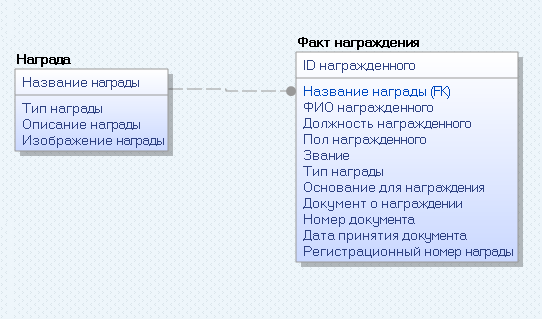
\includegraphics[width=150mm]{pic/er_naive.png}
  \caption{ER-модель объектов предметной области}
  \label{fig:er_naive}
\end{figure}

Нетрудно заметить, что данная модель обладает следующими недостатками:
\begin{itemize}
\item
  дублиование данных: данные о каждом документе,
  подтверждающем факт награждения
  (\textbf{<<документ о награждении>>}, \textbf{<<номер документа>>}, 
  \textbf{<<дата принятия документа>>}) многократно дублируются и хранятся столько раз,
  сколько имеется объектов \textbf{<<факт награждения>>};
\item
  аномалия удаления: при удалении объекта \textbf{<<награда>>} удаляются все сведения
  о лицах, которые были её награждены;
\item
  аномалия обновления: при изменении значения аттрибута \textbf{<<тип награды>>} в объекте
  <<награда>> появляется необходимость изме
\end{itemize}

\subsection{Даталогическое проектирование}
\label{ssub:db_data_stage}

Результатом данного этапа является \textit{схема базы данных}, рассчитанная на конкретную СУБД,
и удовлетворяющая следующим требованиям:
\begin{itemize}
  \item минимальная избыточность хранимых данных;
  \item минимальный физический объем данных;
  \item минимальное время доступа к данным;
  \item сокращение риска потери или искажения данных про внесении изменений в БД.
\end{itemize}

Для того, чтобы удовлетворить приведенные выше требования, достаточно проверить факт нахождения отношений базы данных
в определенной (как минимум, третьей) нормальной форме.
В том случае, когда отношение не отвечает требованиям определенной нормальной формы,
необходимо провести процедуру нормализации отношения.

\textit{Нормализацией отношений} базы данных называется процесс приведения каждого отношения (таблицы) этой базы данных
к определенной нормальной форме. Нормализация каждого отношения выполняется поэтапно: сначала отношение приводится
к первой нормальной форме, затем --- ко второй, и~т.~д.
При переходе к каждой последующей нормальной форме устраняются недостатки
(\textit{аномалии}), присущие предыдущей нормальной форме.

Приведем формальные определения первых трех нормальных форм, взятые из авторитетного источника~\cite{date05}.

Переменная отношения находится в \textit{первой нормальной форме} тогда
и только тогда, когда в любом допустимом значении этой переменной отношения каждый
ее кортеж содержит только одно значение для каждого из атрибутов.

Переменная отношения находится во \textit{второй нормальной форме} тогда и только тогда,
когда она находится в первой нормальной форме и каждый неключевой атрибут
неприводимо зависит от ее первичного ключа.

Переменная отношения находится в \textit{третьей нормальной форме} тогда и только тогда,
когда она находится во второй нормальной форме и ни один неключевой атрибут не является
транзитивно зависимым от ее первичного ключа.

Следует отметить, что существуют также нормальные формы более высоких порядков,
но они редко используются в практических целях.  

\begin{itemize}
\item \textbf{<<факт награждения>>} --- хранит информацию о каждом факте награждения
  конкретного лица конкретной наградой;
\item \textbf{<<награда>>} --- хранит информацию о видах государственных наград
  Республики Беларусь;
\item \textbf{<<награжденный>>} --- хранит информацию о лице, предоставленным
  к государственной награде
\item \textbf{<<документ о награждении>>} --- хранит информацию о документах,
  в которых перечислены списки лиц, предоставленных к награде.
\end{itemize}

Рассмотрим связи между объектами предметной области.
Объект \textbf{<<награжденный>>} может быть связан с несколькими
объектами \textbf{<<факт награждения>>}.
Одному объекту \textbf{<<документ о награждении>>} может соответствовать несколько
объектов \textbf{<<факт награждения>>}.
Наконец, одному объекту \textbf{<<награда>>} может соответствовать несколько объектов
\textbf{<<факт награждения>>}.

Проектируемый сервис должен поддерживать учетные записи администраторов сервиса.
Cведения об учетных записях администраторов разумно
расположить в базе данных. Введем новый объект \textbf{<<учетная запись>>}.
Объект \textbf{<<учетная запись>>} содержит следующие аттрибуты:
имя пользователя, пароль (в зашифрованном виде), адрес электронной почты.

ER-модель проектируемой базы данных приведена на рисунке~\ref{fig:er_final}.

\begin{figure}[h]
  \centering
  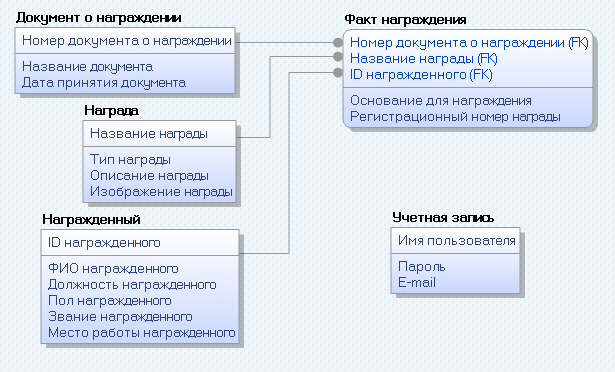
\includegraphics[width=150mm]{pic/er_final.png}
  \caption{ER-модель базы данных проектіруемого веб-сервиса}
  \label{fig:er_final}
\end{figure}


\subsection{Физическое проектирование}
\label{ssub:db_physical_stage}


% \subsection{Нормализация базы данных}
% \label{ssub:db_structure_forms}



% Перечислить определения НФ. Сослаться на тот факт, что ER-модели позволяют автоматически
% получать БД в подходящей НФ.

% \subsection{Проектирование баз данных на основе ER-моделей}
% \label{ssub:db_structure_er_models}


% \subsection{Преобразование ER-моделей в структуру базы данных}
% \label{ssub:db_structure_convert_models_to_structure}


% \subsection{Проектирование базы данных сервиса nagrady.by}
% \label{ssec:db_structure_nagrady}

% В этом подразделе необходимо описать процесс проектирования БД:
% описание содержимого таблиц и связей между ними.
\message{ !name(db_structure.tex) !offset(-373) }
